\documentclass[12pt]{article}

\usepackage{amssymb,amsmath,amsthm} 
\usepackage{graphicx}               

\title{Homework 1}
\author{Jacob Hurst}
\date{\today}
\begin{document}

\maketitle
\clearpage

\section{Question 1: Git Commands}

\subsection{Details}
\begin{enumerate}

\item Execute the command \emph{git log} and find the two most recent commits. Then, execute the command \emph{git diff hash-from-last-commit hash-from-two-commits-ago}. Observe the output. Describe in a few sentences what the command is doing.
\item Modify test.txt, then execute \emph{git diff}. Observe the output. Describe in a few sentences what the command is doing.

\end{enumerate}

\subsection{Results}

\begin{enumerate}

\item The command \emph{git diff tag1 tag2} first determines what changes have occurred in my repository between the two supplied tags. Then, for each change within a file, displays results from a comparison test between the two files that have differences. 

In figure 1, the noticed change is between versions of my hw1/README.md. A line by line comparison of these two files is then displayed. Lines prefixed with \emph{'-'} indicate lines that have been removed from the latest version. Lines prefixed with \emph{'+'} indicate lines that have been added since the last version. Lines without either of these, have not changed.

\item The command \emph{git diff} when not provided tags to compare, compares the most recent local version with the most recent repository version. As with diff1.txt, line by line comparisons are made between each differing file between tags. 

In figure 2, \emph{git diff} noticed changes between test.txt on the local version and the repository version. The \emph{'+'} indicates that the line "Adding a line" was added to the bottom of the test.txt file.

\end{enumerate}

\subsection{Figures}
\begin{figure}[htb]
\begin{center}
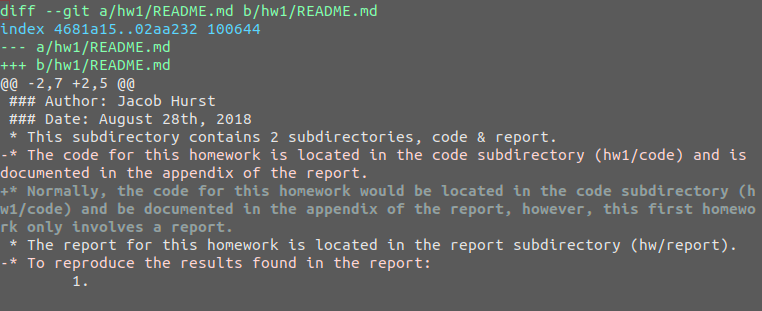
\includegraphics[width=0.9\textwidth]{diff1.png}
   \caption{This figure displays output from git diff hash1 hash2.} 
    \label{fig:1}
\end{center}

\end{figure}
\begin{figure}[htb]
\begin{center}
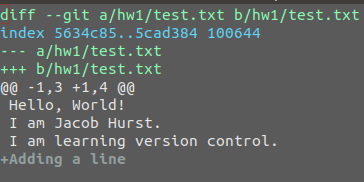
\includegraphics[width=0.9\textwidth]{diff2.png}
   \caption{This figure displays output from git diff.} 
    \label{fig:2}
\end{center}
\end{figure}

\end{document} 

